\documentclass[11pt]{article}
\usepackage{algorithm2e}
\usepackage[italian]{babel}
\usepackage[document]{ragged2e}
\usepackage{amsfonts, amssymb, amsmath}
\usepackage{cancel}
\usepackage{float}
\usepackage{mathtools}
\usepackage[margin=3cm]{geometry}

\tolerance=1
\emergencystretch=\maxdimen
\hyphenpenalty=10000
\hbadness=10000

\begin{document}
\begin{titlepage}
    \begin{center}
        \vspace*{1.5cm}
            
        \Huge
        \textbf{Tweet Analysis}
            
        \vspace{0.3cm}
        \LARGE
        Sprint 1\\[0.2em]
        \Large
        19 novembre 2022 -- 2 novembre 2022

        \vspace{1.5cm}
          
        \begin{minipage}[t]{0.47\textwidth}
            \begin{center}
                \parbox{50mm}{\centering\large {\bf Cheikh Ibrahim $\cdot$ Zaid} \\[0.2em] PO Operativo \\[0.3em] Matricola: \texttt{0000974909}}\\[2em]
                \parbox{50mm}{\centering\large {\bf Lee $\cdot$ Qun Hao Henry} \\[0.2em] Developer \\[0.3em] Matricola: \texttt{0000990259}}
            \end{center}
		\end{minipage}
		\hfill
		\begin{minipage}[t]{0.47\textwidth}\raggedleft
            \begin{center}
                \parbox{50mm}{\centering\large {\bf Xia $\cdot$ Tian Cheng} \\[0.2em] Scrum master \\[0.3em] Matricola: \texttt{0000975129}}\\[2em]
                \parbox{50mm}{\centering\large {\bf Paris $\cdot$ Manuel} \\[0.2em] Developer \\[0.3em] Matricola: \texttt{0000997526}}
            \end{center}
		\end{minipage}  
            
        \vspace{6cm}
            
        Anno accademico\\
        $2022 - 2023$
            
        \vspace{0.8cm}
            
            
        \Large
        Corso di Ingegneria del Software\\
        Alma Mater Studiorum $\cdot$ Università di Bologna\\
            
    \end{center}
\end{titlepage}
\pagebreak


\section*{Sprint goal}
\justify
L'obiettivo dello sprint è stato principalmente quello di studiare le API di Twitter e produrre le prime funzionalità per la visualizzazione e l'analisi dei tweet.\\
In particolare le funzionalità pianificate per lo sprint riguardano:
\begin{itemize}
    \item La ricerca di tweet per username
    \item La ricerca di tweet per hashtag
    \item L'analisi dei tweet tramite componenti grafiche (grafico a torta per il sentiment analysis, grafico a barre per la frequenza dei tweet e word cloud)
\end{itemize}
\begin{figure}[H]
    \centering
    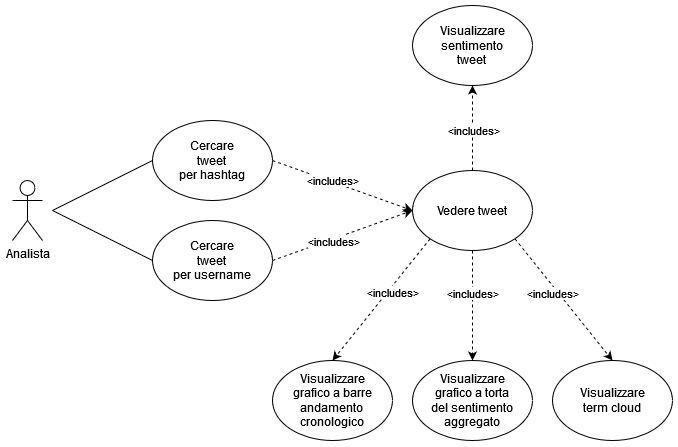
\includegraphics[width=12cm]{./img/usecase.png}
    \caption{Use case previsto per lo sprint 1}
\end{figure}


\newpage
\section*{Team building}
Nel corso dello sprint è stata effettuata una sessione di team building con il gioco \textit{Escape the Boom}.
L'obiettivo era migliorare la comunicazione del team e consolidare i ruoli di ciascuno.\\
La partita è stata valutata positivamente dal team ed è risultata utile per gli scopi per cui era stata pianificata.


\section*{Retrospettiva}
\subsection*{Pre-retrospettiva}
Alla pre-retrospettiva effettuata a metà sprint, sono emerse le seguenti problematiche:
\begin{itemize}
    \item Tempo di lavoro non sufficiente
    \item Mancanza di comunicazione nel team
    \item Task e user stories hanno descrizioni poco dettagliate e facilmente fraintendibili
\end{itemize}
\begin{figure}[H]
    \centering
    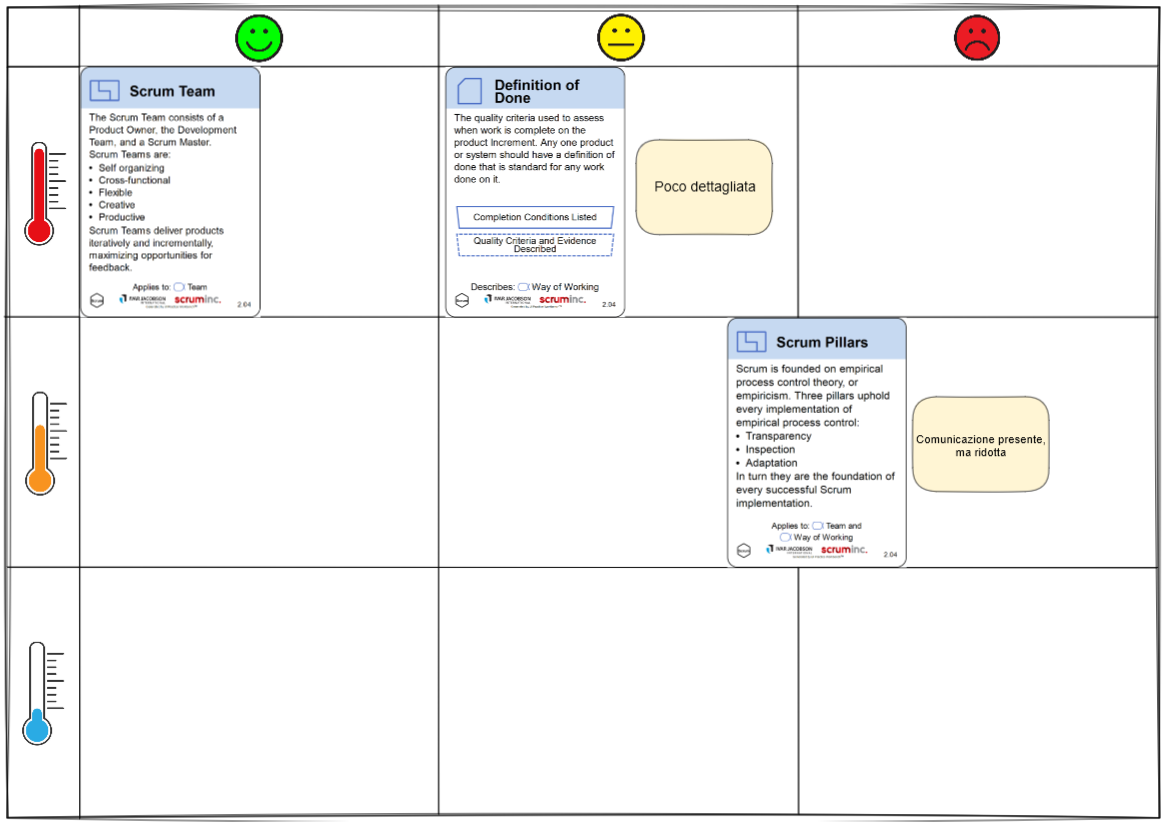
\includegraphics[width=12cm]{./img/preretrospettiva.png}
    \caption{Carte Essence giocate alla pre-retrospettiva}
\end{figure}

\newpage
\subsection*{Retrospettiva}
Alla retrospettiva di fine sprint, gli aspetti positivi evidenziati dal team sono:
\begin{itemize}
    \item Il deliverable presentato alla sprint review è risultato adeguato e funzionante
    \item Il team e i ruoli di ciascuno sono ben definiti
\end{itemize}
Sono invece stati portati all'attenzione del team i seguenti problemi:
\begin{itemize}
    \item Non è stato effettuato un monitoraggio delle ore di lavoro
    \item I problemi evidenziali alla pre-retrospettiva non sono ancora stati risolti 
\end{itemize}
\begin{figure}[H]
    \centering
    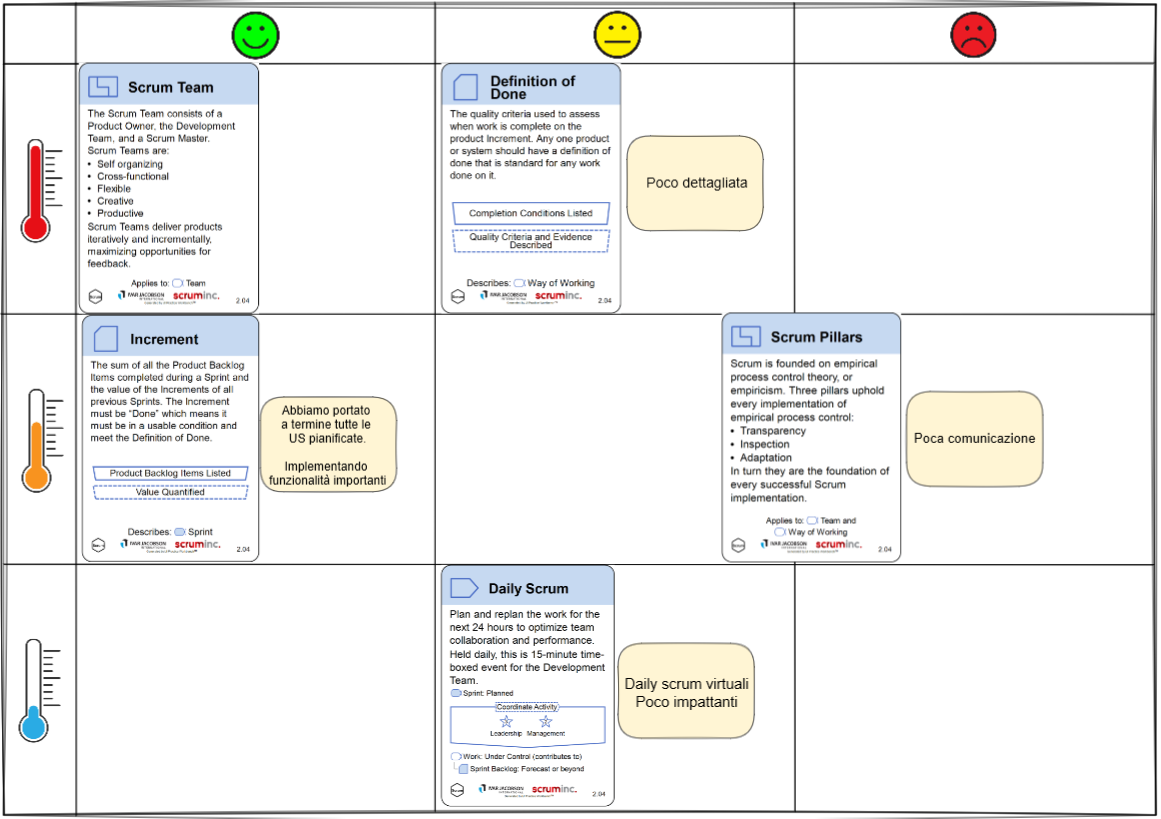
\includegraphics[width=12cm]{./img/retrospettiva.png}
    \caption{Carte Essence giocate alla retrospettiva}
\end{figure}


\end{document}

